\documentclass[spanish]{extbook}
\usepackage[T1]{fontenc}
\usepackage[utf8]{inputenc}
%\usepackage[a4paper,showframe]{geometry}
\usepackage[a4paper]{geometry}
\usepackage{color}
\usepackage{amsmath}
\usepackage{graphicx}
\usepackage{listings}
\usepackage{float}
\usepackage[font=small,labelfont=bf]{caption}
\usepackage{graphicx}
\usepackage{parskip}
\usepackage[hidelinks]{hyperref}
\usepackage[capitalise]{cleveref}
\usepackage{bookmark}
\usepackage[spanish]{babel}
\usepackage{times}
\usepackage{color}

% for adjustwidth environment
\usepackage[strict]{changepage}

% for formal definitions
\usepackage{framed}

% environment derived from framed.sty: see leftbar environment definition
\definecolor{formalshade}{rgb}{0.95,0.95,1}
\definecolor{darkblue}{rgb}{0.0, 0.0, 0.55}

\newenvironment{tradnote}{%
  \def\FrameCommand{%
    \hspace{1pt}%
    {\color{darkblue}\vrule width 2pt}%
    {\color{formalshade}\vrule width 4pt}%
    \colorbox{formalshade}%
  }%
  \vspace{12pt}
  \MakeFramed{\advance\hsize-\width\FrameRestore}%
  \noindent\hspace{-4.55pt}% disable indenting first paragraph
  \begin{adjustwidth}{}{7pt}%
  \vspace{1pt}%
  \textbf{Nota del Traductor:\\}%
}
{%
  \vspace{6pt}\end{adjustwidth}\endMakeFramed%
}


\definecolor{gray97}{gray}{.97}
\definecolor{gray75}{gray}{.75}
\definecolor{gray45}{gray}{.45}

\crefdefaultlabelformat{\textbf{#2#1#3}}
\crefname{figure}{\textbf{Fig.}}{\textbf{Figures}}

\geometry{verbose}
\makeatletter
\numberwithin{equation}{section}
\numberwithin{figure}{section}
\makeatother
\addto\shorthandsspanish{\spanishdeactivate{~<>}}
\renewcommand{\lstlistingname}{Listado de código}
\setlength{\parindent}{0pt}
\renewcommand{\baselinestretch}{0.96}

\usepackage{listings}
\lstset{ frame=Ltb,
     framerule=0pt,
     aboveskip=0.5cm,
     framextopmargin=3pt,
     framexbottommargin=3pt,
     framexleftmargin=0.4cm,
     framesep=0pt,
     rulesep=.4pt,
     backgroundcolor=\color{gray97},
     rulesepcolor=\color{black},
     %
     stringstyle=\ttfamily,
     showstringspaces = false,
     basicstyle=\small\ttfamily,
     commentstyle=\color{gray45},
     keywordstyle=\bfseries,
     %
     numbers=left,
     numbersep=15pt,
     numberstyle=\tiny,
     numberfirstline = false,
     breaklines=true,
   }
 
% minimizar fragmentado de listados
\lstnewenvironment{listing}[1][]
   {\lstset{#1}\pagebreak[0]}{\pagebreak[0]}
 
\lstdefinestyle{consola}
   {basicstyle=\scriptsize\bf\ttfamily,
    backgroundcolor=\color{gray75},
   }
 
\lstdefinestyle{R}
   {language=R,
   }

\title{Introducción a las estadísticas con R}
\date{2018-01-20}
\author{Peter Daalgard\\\small{Traducido al español por Patricio Moracho}}
\begin{document}
\maketitle
% \cleardoublepage
% \pdfbookmark{\contentsname}{Contenido}
% \tableofcontents

%%%%%%%%%%%%%%%%%%%%%%%%%%%%%%%%%%%%%%%%%%%%%%%%%%%%%%%%%%%%%%%%%%%%%%%%%%%%%%%
%% Prefacio
%%%%%%%%%%%%%%%%%%%%%%%%%%%%%%%%%%%%%%%%%%%%%%%%%%%%%%%%%%%%%%%%%%%%%%%%%%%%%%%
\chapter*{Prefacio}

\textbf{R} es un programa informático para estadístas, disponible a través de
Internet bajo la Licencia Pública General (\textbf{GPL}). Es decir, se
suministra con una licencia que nos permite utilizarlo libremente, distribuirlo
o incluso venderlo, siempre que el receptor tenga los mismos derechos y el
código fuente esté disponible libremente. Existen versiones para Microsoft
Windows XP o posteriores, para una variedad de plataformas Unix y Linux, y para
Apple Macintosh OS X. 

\textbf{R} proporciona un entorno en el que puede realizar análisis
estadísticos y producir gráficos.  En realidad es un lenguaje de programación
completo, aunque eso, en este libro sólo se describe marginalmente. Aquí nos
conformamos con aprender los conceptos elementales y ver varios ejemplos. 

\textbf{R} está diseñado de tal manera que siempre es posible realizar más
cálculos sobre los resultados de un procedimiento estadístico. Además, la
funcionalidad para la presentación gráfica de los datos permite tanto métodos
simples, como por ejemplo \texttt{plot(x, y)}, como también la posibilidad de
un control mucho más fino del aspecto de las gráficas. 

El hecho que \textbf{R} esté basado en un lenguaje formal de computadora le da
una tremenda flexibilidad.  Otros sistemas presentan interfaces más sencillas
en términos de menús y formularios, pero a menudo la aparente facilidad de uso
se convierte en un obstáculo a largo plazo. Aunque las estadísticas elementales
se presentan a menudo como una colección de procedimientos fijos, el análisis
de datos moderadamente complejos requiere la creación de modelos estadísticos
ad-hoc, lo que hace que la flexibilidad añadida de \textbf{R} sea altamente
deseable.

\textbf{R} debe su nombre a una típica humorada de Internet. Es posible que
haya oido hablar del lenguaje de programación C (cuyo nombre es otra historia
en sí misma). Inspirados por esto, Becker y Chambers eligieron, a principios de
los años ochenta, llamar a su nuevo lenguaje de programación estadística S.
Este lenguaje se desarrolló aún más con el producto comercial S-PLUS, que a
finales de la década era de uso generalizado entre los estadísticos de todo
tipo. Ross Ihaka y Robert Gentleman de la Universidad de Auckland, Nueva
Zelanda, eligieron escribir una versión reducida de S para propósitos de
enseñanza, y ¿qué era más natural que elegir la letra inmediatamente anterior?
Las iniciales de Ross y Robert también pueden haber jugado un papel importante
en la elección del nombre.

En 1995, Martin Maechler persuadió a Ross y Robert para que publicaran el
código fuente de \textbf{R} bajo la licencia \textbf{GPL}. Esto coincidió con
el auge del software de código abierto impulsado por el sistema Linux. R pronto
logró llenar un hueco en gente como yo que tenía la intención de usar Linux
para computación estadística, pero no tenía ningún paquete estadístico
disponible en ese momento. Se creó una lista de correo para la comunicación de
informes de fallos y discusiones sobre el desarrollo de \textbf{R}.

En agosto de 1997, me invitaron a unirme a un equipo internacional extendido
cuyos miembros colaboran a través de Internet y que ha controlado el desarrollo
de \textbf{R} desde entonces. Posteriormente, el equipo básico se amplió varias
veces y actualmente cuenta con 19 miembros. El 29 de febrero de 2000, se
publicó la versión 1.0.0.0. Al momento de este escrito, la versión actual es
la 2.6.2. Este libro se basó originalmente en una serie de notas elaboradas
para el curso de Estadística Básica para Investigadores en Salud de la Facultad
de Ciencias de la Salud de la Universidad de Copenhague. El curso tenía como
objetivo principal, los estudiantes del doctorado en medicina. Sin embargo, el
material se ha revisado sustancialmente y espero que sea útil para un público
más amplio, aunque sigue habiendo algunos sesgos bioestadísticos, especialmente
en la elección de ejemplos. En los últimos años, el curso de Práctica
Estadística en Epidemiología, que se ha celebrado anualmente en Tartu
(Estonia), ha sido una fuente importante de inspiración y experiencia en la
introducción de jóvenes estadísticos y epidemiólogos a \textbf{R}.  Este libro
no es un manual para \textbf{R}.  La idea es introducir una serie de conceptos
y técnicas básicas que deberían permitir al lector comenzar con estadísticas
prácticas. En cuanto a los métodos prácticos, el libro cubre una currícula
razonable para los estudiantes de primer año de estadística teórica, así como
para los estudiantes de ingeniería. Estos grupos eventualmente necesitarán ir
más allá y estudiar modelos más complejos, así como técnicas generales que
involucren programación real en el lenguaje \textbf{R}.

Para los áreas en las que las estadísticas elementales se enseñan
principalmente como una herramienta, el libro va un poco más allá de lo que se
enseña comúnmente a nivel universitario. Los métodos de regresión múltiple o el
análisis de experimentos multifactoriales rara vez se enseñan a ese nivel, pero
pueden convertirse rápidamente en esenciales para la investigación práctica. He
recopilado los métodos más simples al principio para hacer el libro más legible
también en un nivel elemental. Sin embargo, para mantener el material técnico
consistente, los capítulos 1 y 2 sí incluyen material que algunos lectores
querrán omitir. Por lo tanto, el libro pretende ser útil para varios grupos,
pero no pretenderé que pueda valerse por sí solo para ninguno de ellos. He
incluido breves secciones teóricas en relación con los diversos métodos, pero
más que como material didáctico, éstos deberían servir de recordatorios o
quizás como aperitivos para los lectores que son nuevos en el mundo de la
estadística.

\cleardoublepage
\pdfbookmark{\contentsname}{Contenido}
\tableofcontents


%%%%%%%%%%%%%%%%%%%%%%%%%%%%%%%%%%%%%%%%%%%%%%%%%%%%%%%%%%%%%%%%%%%%%%%%%%%%%%%
%% Conceptos Básicos
%%%%%%%%%%%%%%%%%%%%%%%%%%%%%%%%%%%%%%%%%%%%%%%%%%%%%%%%%%%%%%%%%%%%%%%%%%%%%%%
\chapter{Conceptos Básicos}

El propósito de este capítulo es que empiece a usar  \textbf{R}.  Asumimos que
ya tiene una instalación funcional del software y del paquete \texttt{ISwR} que
contiene los conjuntos de datos para este libro. Las instrucciones para obtener
e instalar el software se encuentran en el \index{Apéndice A}. Como ya
mencionamos, el libro describe la versión 2.6.2 de  \textbf{R}.  En la medida
de lo posible, presento los temas de una manera que es independiente del
sistema operativo en uso y asumo que el lector tiene el conocimiento operativo
elemental para seleccionar desde menús, mover ventanas, etc. Sin embargo, hago
excepciones cuando soy consciente de dificultades específicas con una
plataforma o características específicas de la misma.

\begin{tradnote} 
	Al momento de la traducción la versión actual de R es la
	3.4.2, aún así, lo ejemplos y el código en general del libro son totalmente
	consistentes con las nuevas versiones. Asimismo es importante notar que el
	autor se centra en la forma estándar y básica de introducir comandos,
	directamente trabajando sobre la consola \textbf{R}, sin embargo, el lector
	puede trabajar con entornos más complejos de desarrollo como
	\textbf{Rstudio} que no debería significar grandes diferencias.
\end{tradnote} \newpage

%%%%%%%%%%%%%%%%%%%%%%%%%%%%%%%%%%%%%%%%%%%%%%%%%%%%%%%%%%%%%%%%%%%%%%%%%%%%%%%
%% Primeros pasos
%%%%%%%%%%%%%%%%%%%%%%%%%%%%%%%%%%%%%%%%%%%%%%%%%%%%%%%%%%%%%%%%%%%%%%%%%%%%%%%
\section{Primeros pasos}

Esta sección ofrece una introducción al entorno informático de  \textbf{R}
Computing y le muestra sus características más básicas. Iniciar  \textbf{R} es
sencillo, pero el método dependerá de su plataforma informática.  Podrá
iniciarlo desde el menú del sistema, haciendo doble clic en un icono o
introduciendo el comando \textquotedbl{}R\textquotedbl{} en la línea de
comandos del sistema. Esto producirá una ventana de consola o hará que
\textbf{R} se inicie como un programa interactivo en la ventana del terminal
actual. 

\begin{figure}[H]
  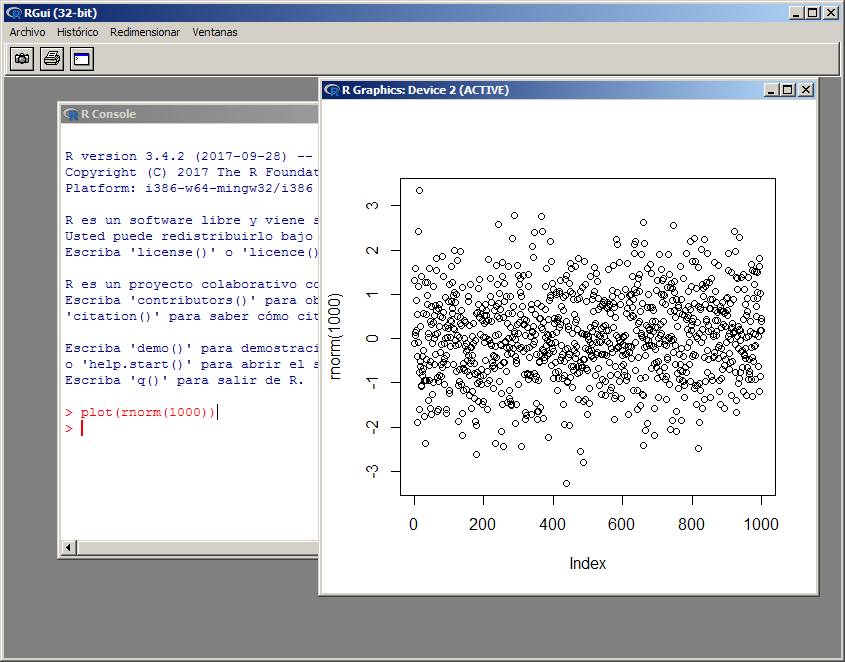
\includegraphics[width=\linewidth]{fig-1.png}
  \caption{Captura de patalla de R Windows.}
  \label{fig:fig-1}
\end{figure}

En cualquier caso, R funciona fundamentalmente según el modelo de
preguntas y respuestas:

Ingrese una línea con un comando y pulse \texttt{<ENTER>} (\texttt{<--}).
Entonces el programa hace algo, imprime el resultado si es relevante y pide más
información.

Cuando \textbf{R} está listo para la entrada, imprime su símbolo, un
\textquotedbl{}>\textquotedbl{}.  Es posible usar \textbf{R} como una
aplicación en modo sólo texto, y también en el modo por lotes, pero para los
propósitos de este capítulo, asumo que usted está sentado en una estación de
trabajo gráfica.

Todos los ejemplos de este libro deberían ejecutarse si los escribes
exactamente como están impresos, siempre y cuando tengas el paquete
\texttt{ISwR} no sólo instalado sino también cargado en tu ruta de búsqueda
actual. Esto se hace introduciendo:
\newpage

\begin{lstlisting}[language=R]
> library(ISwR)
\end{lstlisting}

en la línea de comandos. No necesita entender lo que hace este comando en este
preciso momento. Se explicará en la Sección 2.1.5. Para una primera impresión de
lo que \textbf{R} puede hacer, intente escribir lo siguiente:

\begin{lstlisting}[language=R]
> plot(rnorm(1000))
\end{lstlisting}

Este comando dibuja 1000 números al azar a partir de la distribución normal
(rnorm = \emph{r}andom \emph{norm}al) y los dibuja en una ventana emergente de
gráficos. El resultado en una máquina Windows se puede ver en la Figura
\ref{fig:fig-1}.  Por supuesto, en este momento no esperamos que adivine que
obtendría este resultado de esa forma en particular. Elegimos este ejemplo
porque muestra varios componentes de la interfaz de usuario en acción. Antes de
que el estilo de comandos sea natural para usted, es necesario introducir
algunos conceptos y convenciones a través de ejemplos más simples. Bajo
Windows, la ventana de gráficos tomará el enfoque del teclado en este punto.
Haga clic en la consola para que acepte más comandos.

%%%%%%%%%%%%%%%%%%%%%%%%%%%%%%%%%%%%%%%%%%%%%%%%%%%%%%%%%%%%%%%%%%%%%%%%%%%%%%%
%% Una calculadora gigante
%%%%%%%%%%%%%%%%%%%%%%%%%%%%%%%%%%%%%%%%%%%%%%%%%%%%%%%%%%%%%%%%%%%%%%%%%%%%%%%
\subsection{Una calculadora gigante}

Una de las tareas más simples y posibles de hacer en \textbf{R} es introducir una
expresión aritmética y obtener un resultado. (La segunda línea es la respuesta
de la máquina.)

\begin{lstlisting}[language=R]
> 2 + 2 
[1] 4
\end{lstlisting}

De esta forma vemos que la máquina sabe que 2 más 2 son 4. Por supuesto,
también sabe hacer otros cálculos estándar, como ser $e^{-2}$:

\begin{lstlisting}[language=R]
> exp(-2) 
[1] 0.1353353
\end{lstlisting}

El \texttt{{[}1{]}} delante del resultado es parte de la forma en
que \textbf{R} imprime números
y vectores. No es útil aquí, pero lo es cuando el resultado es un
vector más largo. El número entre corchetes es el índice del primer
número de esa línea. Considere el caso de generar 15 números aleatorios
a partir de una distribución normal:

\begin{lstlisting}[language=R]
> rnorm(15) 
[1]  -0.18326112 -0.59753287 -0.67017905 0.16075723  1.28199575
[6]   0.07976977  0.13683303  0.77155246 0.85986694 -1.01506772
[11] -0.49448567  0.52433026  1.07732656 1.09748097 -1.09318582
\end{lstlisting}

Aquí, por ejemplo, el \texttt{{[}6{]}} indica que\texttt{ 0.07976977}
es el sexto elemento del vector. (Por razones tipográficas, los ejemplos
en este libro están hechos con un ancho de línea acortado. Si lo prueba
en su propia máquina, verá los valores impresos con seis números por
línea en lugar de cinco. Los números en sí mismos también serán diferentes
ya que se trata justamente de una generación de números aleatoria.

\begin{tradnote} Hay un mecanismo para asegurar que una generación aleatoria
sea consistente en distintos momentos y es la de establecer un ``semilla''
incial con que se ejecutarán cualquier rutina aleatoria, esto se logra mediante
la ejecución de \texttt{set.seed(<número>)}, el \texttt{<número>}, no importa
cual, es lo que hace repetible y consistente los datos aleatorios\end{tradnote} 

\subsection{Asignaciones}

Incluso en una calculadora, usted necesitará eventualmente una manera de
almacenar resultados intermedios, de modo que no tenga que ingresarlos una y
otra vez. \textbf{R}, al igual que otros lenguajes informáticos, tiene
variables simbólicas, es decir, nombres que se pueden utilizar para representar
valores. Para asignar el valor 2 a la variable x, se puede introducir:

\begin{lstlisting}[language=R]
> x <- 2
\end{lstlisting}


Los dos caracteres \texttt{<-} deben leerse como un solo símbolo: una flecha
que señala la variable a la que se asigna el valor. Esto se conoce como el
operador de asignación. El espaciamiento alrededor de los operadores es
generalmente ignorado por \textbf{R}, pero note que agregar un espacio en medio
de un <- cambia el significado a \textquotedbl{}menos que\textquotedbl{}
seguido por \textquotedbl{}menos\textquotedbl{} (¡a la inversa, omitir el
espacio al comparar una variable con un número negativo tiene consecuencias
inesperadas!). 

\begin{tradnote}
	Es importante hacer notar, que si bien, por motivos históricos
	el operador de asignación es \texttt{<-}, \textbf{R} permite la definir una asignación
	de la forma habitual en otros lenguajes, mediante el operador de igualdad (\texttt{=}),
	sin embargo en la práctica es mucho más habitual ver la asignaciones
	escritas mediante \texttt{<-}.
\end{tradnote} 

No hay un resultado inmediatamente visible, pero a partir de ahora,
\texttt{x} tiene el valor 2 y puede ser utilizado en las siguientes
expresiones aritméticas.

\begin{lstlisting}[language=R]
> x 
[1] 2 
> x + x 
[1] 4
\end{lstlisting}

Los nombres de las variables pueden elegirse libremente en \textbf{R}.  Pueden
construirse a partir de letras, dígitos y el símbolo de punto.  Sin embargo,
existe la limitación de que el nombre no debe comenzar con un dígito o un punto
seguido de un dígito. Los nombres que comienzan con un punto son especiales y
deben evitarse. Un nombre de variable típico podría ser \texttt{height.1yr},
que podría utilizarse para describir la altura de un niño a la edad de 1 año.
Los nombres son sensibles a mayúsculas y minúsculas: \texttt{WT} y \texttt{wt}
no se refieren a la misma variable.

El sistema ya utiliza algunos nombres. Esto puede causar cierta confusión si
los utiliza para otros fines. Los peores casos son los nombres de una sola
letra \texttt{c}, \texttt{q}, \texttt{t}, \texttt{C}, \texttt{D}, \texttt{F},
\texttt{I}, y \texttt{T}, pero también hay otros como \texttt{diff},
\texttt{df}, y \texttt{pt}, por ejemplo.  La mayoría de éstas son funciones y
no suelen causar problemas cuando se utilizan como nombres de variables. Sin
embargo, \texttt{F} y \texttt{T} son las abreviaturas estándar de
\texttt{FALSE} y \texttt{TRUE} y ya no funcionan como tales si las redefine.

\subsection{Aritmetica vectorizada}

No se pueden hacer muchas estadísticas sobre números individuales!  Más bien,
por ejemplo, usted examinará los datos de un grupo de pacientes.  Una de las
fortalezas de \textbf{R} es que puede manejar vectores de datos enteros como
objetos individuales.  Un vector de datos es simplemente un arreglo de números,
y una variable vectorial puede ser construida así:

\begin{lstlisting}[language=R]
> weight <- c(60, 72, 57, 90, 95, 72) 
> weight 
[1] 60 72 57 90 95 72
\end{lstlisting}

La clausula \texttt{c(...)} se utiliza para definir vectores. Los números son
inventados, pero podrían representar los pesos (en kg) de un grupo de hombres
normales. Esta no es la única manera de introducir vectores de datos en
\textbf{R} ni siquiera es el método preferido, pero los vectores simples como
el anterior se usan para muchos otros propósitos, y la construcción
\texttt{c(...)} se usa extensivamente. En la Sección 2.4, discutimos técnicas
alternativas para la lectura de datos. Por ahora, nos atenemos a un único
método. Se pueden hacer cálculos con vectores igual que los números ordinarios,
siempre y cuando tengan la misma longitud.  Supongamos que también tenemos las
alturas que corresponden a los pesos anteriores. El índice de masa corporal
(IMC) o ``body mass index'', se define para cada persona como el peso en
kilogramos dividido por el cuadrado de la altura en metros. Esto podría
calcularse de la siguiente manera:

\begin{lstlisting}[language=R]
> height <- c(1.75, 1.80, 1.65, 1.90, 1.74, 1.91) 
> bmi <- weight/height^2 
> bmi 
[1] 19.59184 22.22222 20.93664 24.93075 31.37799 19.73630
\end{lstlisting}

Tenga en cuenta que la operación se lleva a cabo elemento por elemento (es
decir, el primer valor de \texttt{bmi} es $60/1.75^2$ y así sucesivamente) y
que el operador \textasciicircum se usa para calcular una potencia. (En algunos
teclados, \textasciicircum es una "tecla muerta" y deberá presionar la barra
espaciadora para que se muestre).

De hecho, es posible realizar operaciones aritméticas sobre vectores de
diferente longitud. Ya lo hemos usado cuando antes calculamos $height^2$
ya que \texttt{2} en definitiva es un vector de longitud 1. En tales casos, el
vector más corto se recicla. Esto se usa principalmente con vectores de
longitud 1 (escalares) pero a veces también en otros casos donde se desea un
patrón de repetición. Tenga en cuenta que se emitirá una advertencia si el
vector más largo no es un múltiplo de menor longitud.

Estas convenciones para los cálculos vectorizados hacen que sea muy fácil
realizar cálculos estadísticos típicos. Considere, por ejemplo, el cálculo
de la media y la desviación estándar de la variable de peso: $\bar{x} = \sum x_1/n$

\begin{lstlisting}[language=R]
> sum(weight)
[1] 446
> sum(weight)/length(weight)
[1] 74.33333
\end{lstlisting}

A continuación, salvamos la media en una variable \texttt{xbar} y continuamos
con el cálculo de la desviación estándar $SD = \sqrt{\sum (x_i -\bar{x})^2/(n)}$. 
Hacemos esto en pasos para ver los componentes individuales. Las desviaciones 
de la media son: 

\begin{lstlisting}[language=R]
> xbar <- sum(weight)/length(weight)
> weight - xbar
[1] -14.333333 -2.333333 -17.333333  15.666667 20.666667
[6] -2.333333 
\end{lstlisting}

Observe cómo \texttt{xbar}, que tiene una longitud de 1, es reciclada y
sustraída de cada elemento de \texttt{weight}. Las desviaciones al cuadrado
serán:

\begin{lstlisting}[language=R]
> (weight - xbar)^2
[1] 205.444444 5.444444 300.444444 245.444444 427.111111
[6] 5.444444
\end{lstlisting}

Como este comando es bastante similar al anterior, es conveniente introducirlo
editando el comando anterior. En la mayoría de los sistemas que ejecutan
\textbf{R}, el comando anterior se puede recuperar con la tecla de flecha hacia
arriba. 

La suma de las desviaciones cuadradas se obtiene del mismo modo con

\begin{lstlisting}[language=R]
> sum((weight - xbar)^2)
[1] 1189.333
\end{lstlisting}

Y entonces la desviación estándar:

\begin{lstlisting}[language=R]
> sqrt(sum((weight - xbar)^2)/(length(weight) - 1))
[1] 15.42293
\end{lstlisting}

Por supuesto, como \textbf{R} es un programa estadístico, estos cálculos ya
están incorporados en el programa, y se obtienen los mismos resultados
simplemente de esta forma:

\begin{lstlisting}[language=R]
> mean(weight)
[1] 74.33333
> sd(weight)
[1] 15.42293
\end{lstlisting}

\subsection{Procedimientos comunes}

Como ejemplo de algo un poco más complicado de lo que \textbf{R} es capaz de
hacer, considere lo siguiente: La regla general es que el IMC (Índice de masa
corporal) para un individuo de peso normal debería estar entre 20 y 25, y
queremos saber si nuestros datos se desvían sistemáticamente de eso. Se puede
utilizar una prueba t de una muestra para evaluar si el IMC de las seis
personas puede considerarse que tiene una media de 22,5, dado que proviene de
una distribución normal. Para ello, puede utilizar la función \texttt{t.test}. (Podría
no conocer la teoría de la prueba t todavía. El ejemplo se incluye aquí
principalmente para dar una indicación de cómo es la producción estadística
``real''. En el capítulo 5 se ofrece una descripción detallada de \texttt{t.test})

%\begin{lstlisting}[language=R]
\begin{lstlisting}[style=R]
> t.test(bmi, mu=22.5)

One Sample t-test
data: bmi
t = 0.3449, df = 5, p-value = 0.7442
alternative hypothesis: true mean is not equal to 22.5
95 percent confidence interval:
18.41734 27.84791
sample estimates:
mean of x
23.13262
\end{lstlisting}

El parametro \texttt{mu=22.5} define el valor de \texttt{mu}, que representa la
letra griega $\mu$ usada convencionalmente para el definir teoricamente la
media. Si este valor no se inidca, \texttt{t.test} usaría  \texttt{mu=0} por
defecto, que no es de interés aquí.  

Para un test como este, obtenemos una salida más extensa que en los ejemplos
anteriores. Los detalles se explican en el capítulo 5, pero es importante poner
el foco en el \texttt{p.value} que se utiliza para probar la hipótesis de que
la media es de 22,5. El valor de \texttt{p.value} no es pequeño, lo que indica
que no es en absoluto improbable obtener datos como los observados si el
promedio fuera de hecho de 22,5. (Hablando de forma poco académica: en realidad
\texttt{p} es la probabilidad de obtener un valor \texttt{t} mayor que 0.3449 o
menor que -0.3449.) Sin embargo, también se puede observar el intervalo de
confianza del 95\% para la media real. Este intervalo es bastante amplio, lo que
indica que tenemos muy poca información sobre el verdadero promedio.
\newpage

\subsection{Gráficos}

Uno de los aspectos más importantes de la presentación y análisis de datos es
la generación de gráficos adecuados. \textbf{R} - como antes \textbf{S} - tiene un modelo
para construir gráficos que permite la producción simple de gráficos estándar,
así como el control fino sobre los componentes del mismo. 

Si quieres investigar la relación entre  \texttt{weight} y \texttt{height}, una
primer aproximación es contrastarlos uno con el otro en una gráfica. Esto se
hace mediante:

\begin{lstlisting}[language=R]
> plot(height,weight)
\end{lstlisting}

\begin{figure}[H]
  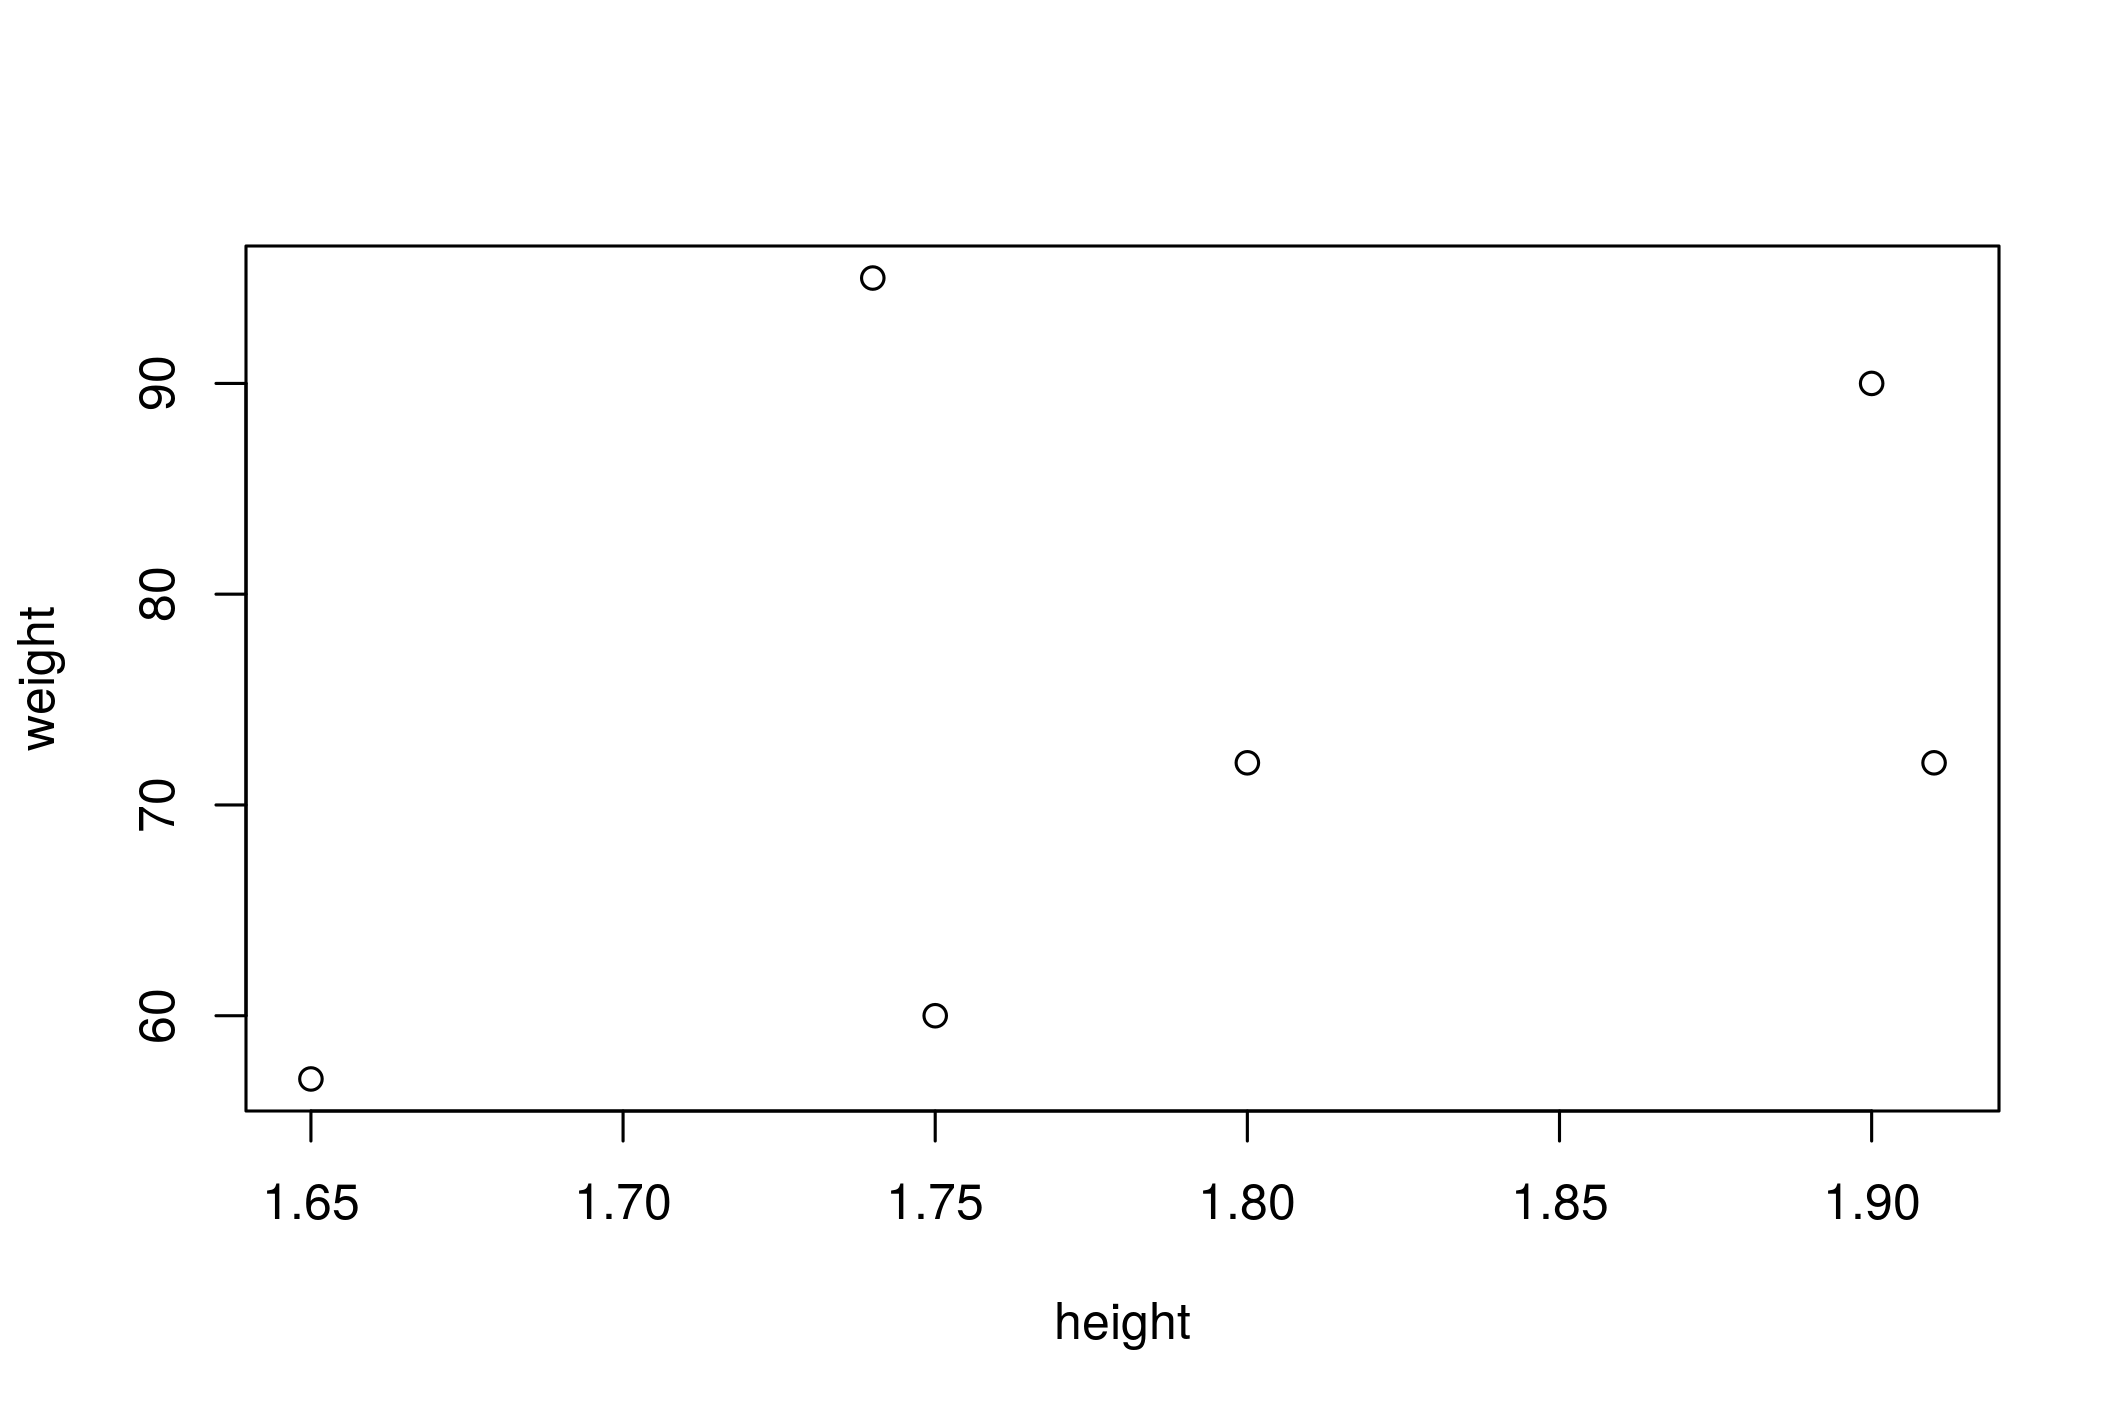
\includegraphics[width=\linewidth]{fig-2.png}
  \caption{Un simple gráfico x-y}
  \label{fig:fig-2}
\end{figure}

Puede modificar el grafico de múltiples formas. Para ello, hay una enorme
cantidad de parámetros que se pueden establecer. Como ejemplo, intentemos
cambiar el símbolo para gráficar cada punto usando la palabra clave
\texttt{pch} ("plotting character") de esta manera:

\begin{lstlisting}[language=R]
> plot(height, weight, pch=2)
\end{lstlisting}

Esto da la gráfica en la Figura \ref{fig:fig-2}, con los puntos marcados ahora
con pequeños triángulos.

La idea detrás del cálculo del IMC es que este valor debe ser independiente de
la estatura de la persona, dando así un número único como indicación de si una
persona tiene sobrepeso y en qué medida. Dado que un IMC normal debe ser de
aproximadamente 22.5, podriamos esperar que $weight \approx 22.5 * height^2$.
De acuerdo a esto podríamos sobreponer una curva del peso esperado para un IMC
de 22.5 de la siguiente forma:

\begin{lstlisting}[language=R]
> hh <- c(1.65, 1.70, 1.75, 1.80, 1.85, 1.90)
> lines(hh, 22.5 * hh^2)
\end{lstlisting}

Lo podremos verificar en la Figura \ref{fig:fig-4}. La función \texttt{lines}
sumará los valores \texttt{(x, y))} para terminar generando una recta en el
gráfico actual.

La razón para definir una nueva variable (\texttt{hh}) para las alturas en
lugar de utilizar el vector original (\texttt{height}) es doble. En primer
lugar, la relación entre altura y peso es cuadrática y por lo tanto no lineal,
aunque puede ser difícil de ver en el gráfico. Puesto que estamos aproximando
una curva no lineal con una curva lineal a intervalos, será mejor utilizar
puntos que estén repartidos uniformemente a lo largo del eje \textit{x} que
confiar en la distribución de los datos originales. En segundo lugar, puesto
que los valores de \texttt{height} no están ordenados, los segmentos de línea
no conecta puntos vecinos, sino que se desplazan hacia adelante y hacia atrás
entre puntos distantes.

%%%%%%%%%%%%%%%%%%%%%%%%%%%%%%%%%%%%%%%%%%%%%%%%%%%%%%%%%%%%%%%%%%%%%%%%%%%%%%%
%% R elementos escenciales del lenguaje
%%%%%%%%%%%%%%%%%%%%%%%%%%%%%%%%%%%%%%%%%%%%%%%%%%%%%%%%%%%%%%%%%%%%%%%%%%%%%%%
\section{R elementos escenciales del lenguaje}

Esta sección describe los aspectos básicos del lenguaje \textbf{R}. Es
necesario hacer esto de una manera ligeramente superficial, con algunos
detalles a los que no profundizaremos demasiado.  El énfasis estará puesto en los
elementos que son útiles conocer para el uso interactivo en lugar de la
programación real , aunque se incluye una breve sección sobre programación.

\subsection{Expresiones y objetos}

La forma básica de interactuar en \textbf{R} es la de evaluación de
expresiones. El usuario introduce una expresión; el sistema la evalúa e imprime
el resultado.  Algunas expresiones se evalúan no por sus resultados sino por
los efectos secundarios tales como poner una ventana de gráficos o escribir en
un archivo. Todas las expresiones R devuelven un valor (posiblemente NULL),
pero a veces ese valor es ``invisible''  y no se imprime valor alguno en la
consola.

\newpage
\begin{figure}[!htb]
	\centering
	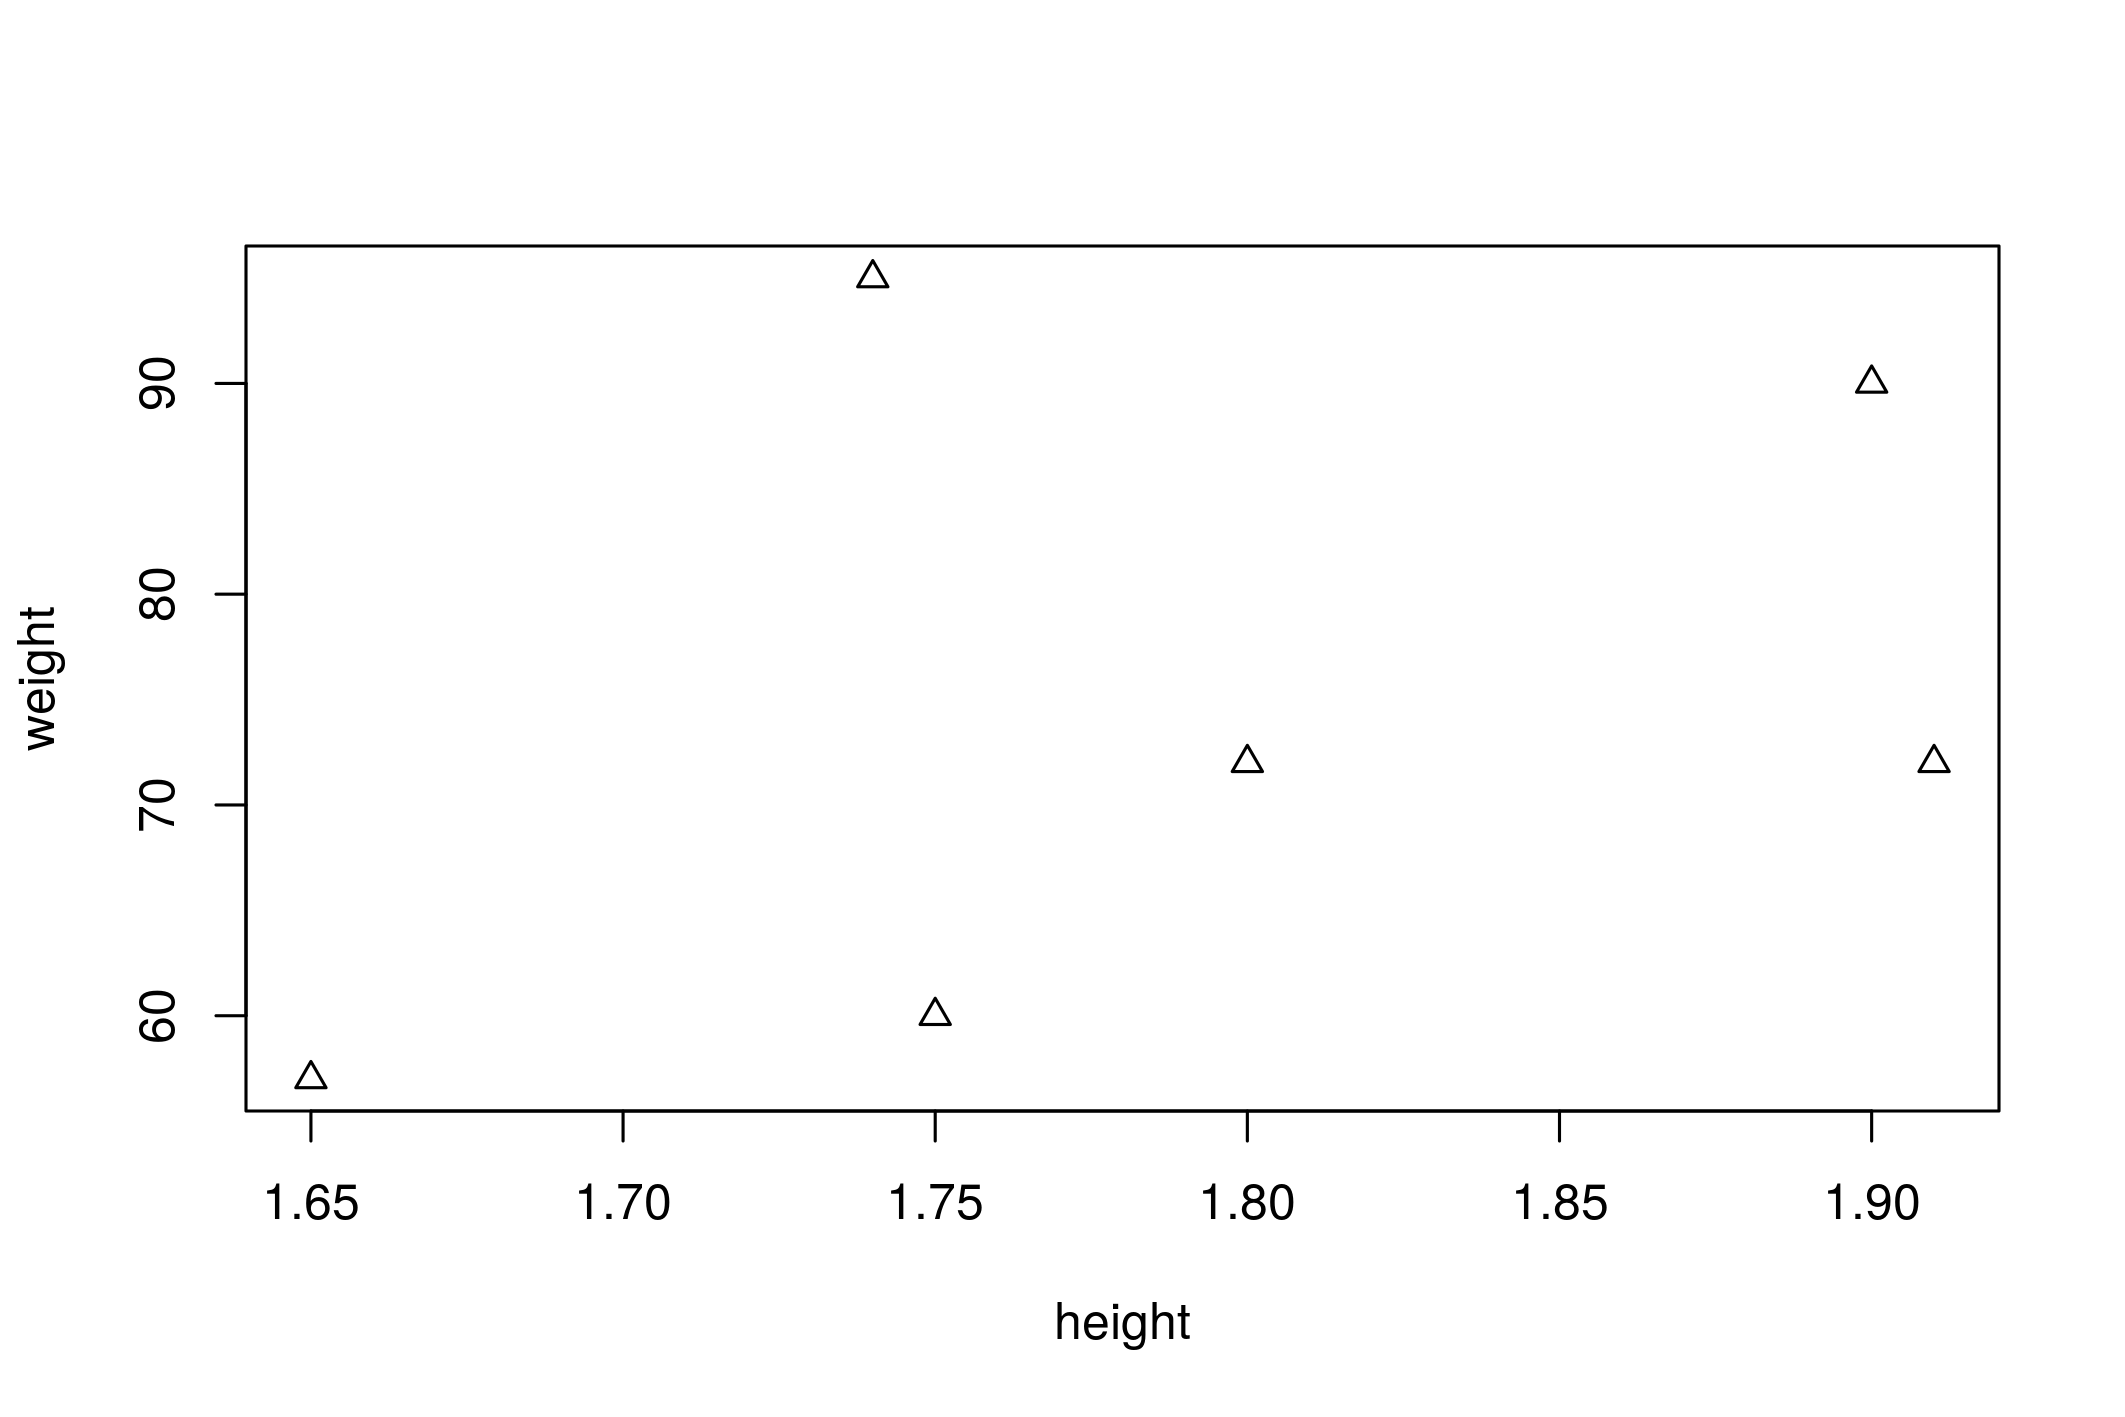
\includegraphics[width=0.95\textwidth]{fig-3.png}
	\caption{Gráfico usando \texttt{pch=2}}
	\label{fig:fig-3}
	\centering
	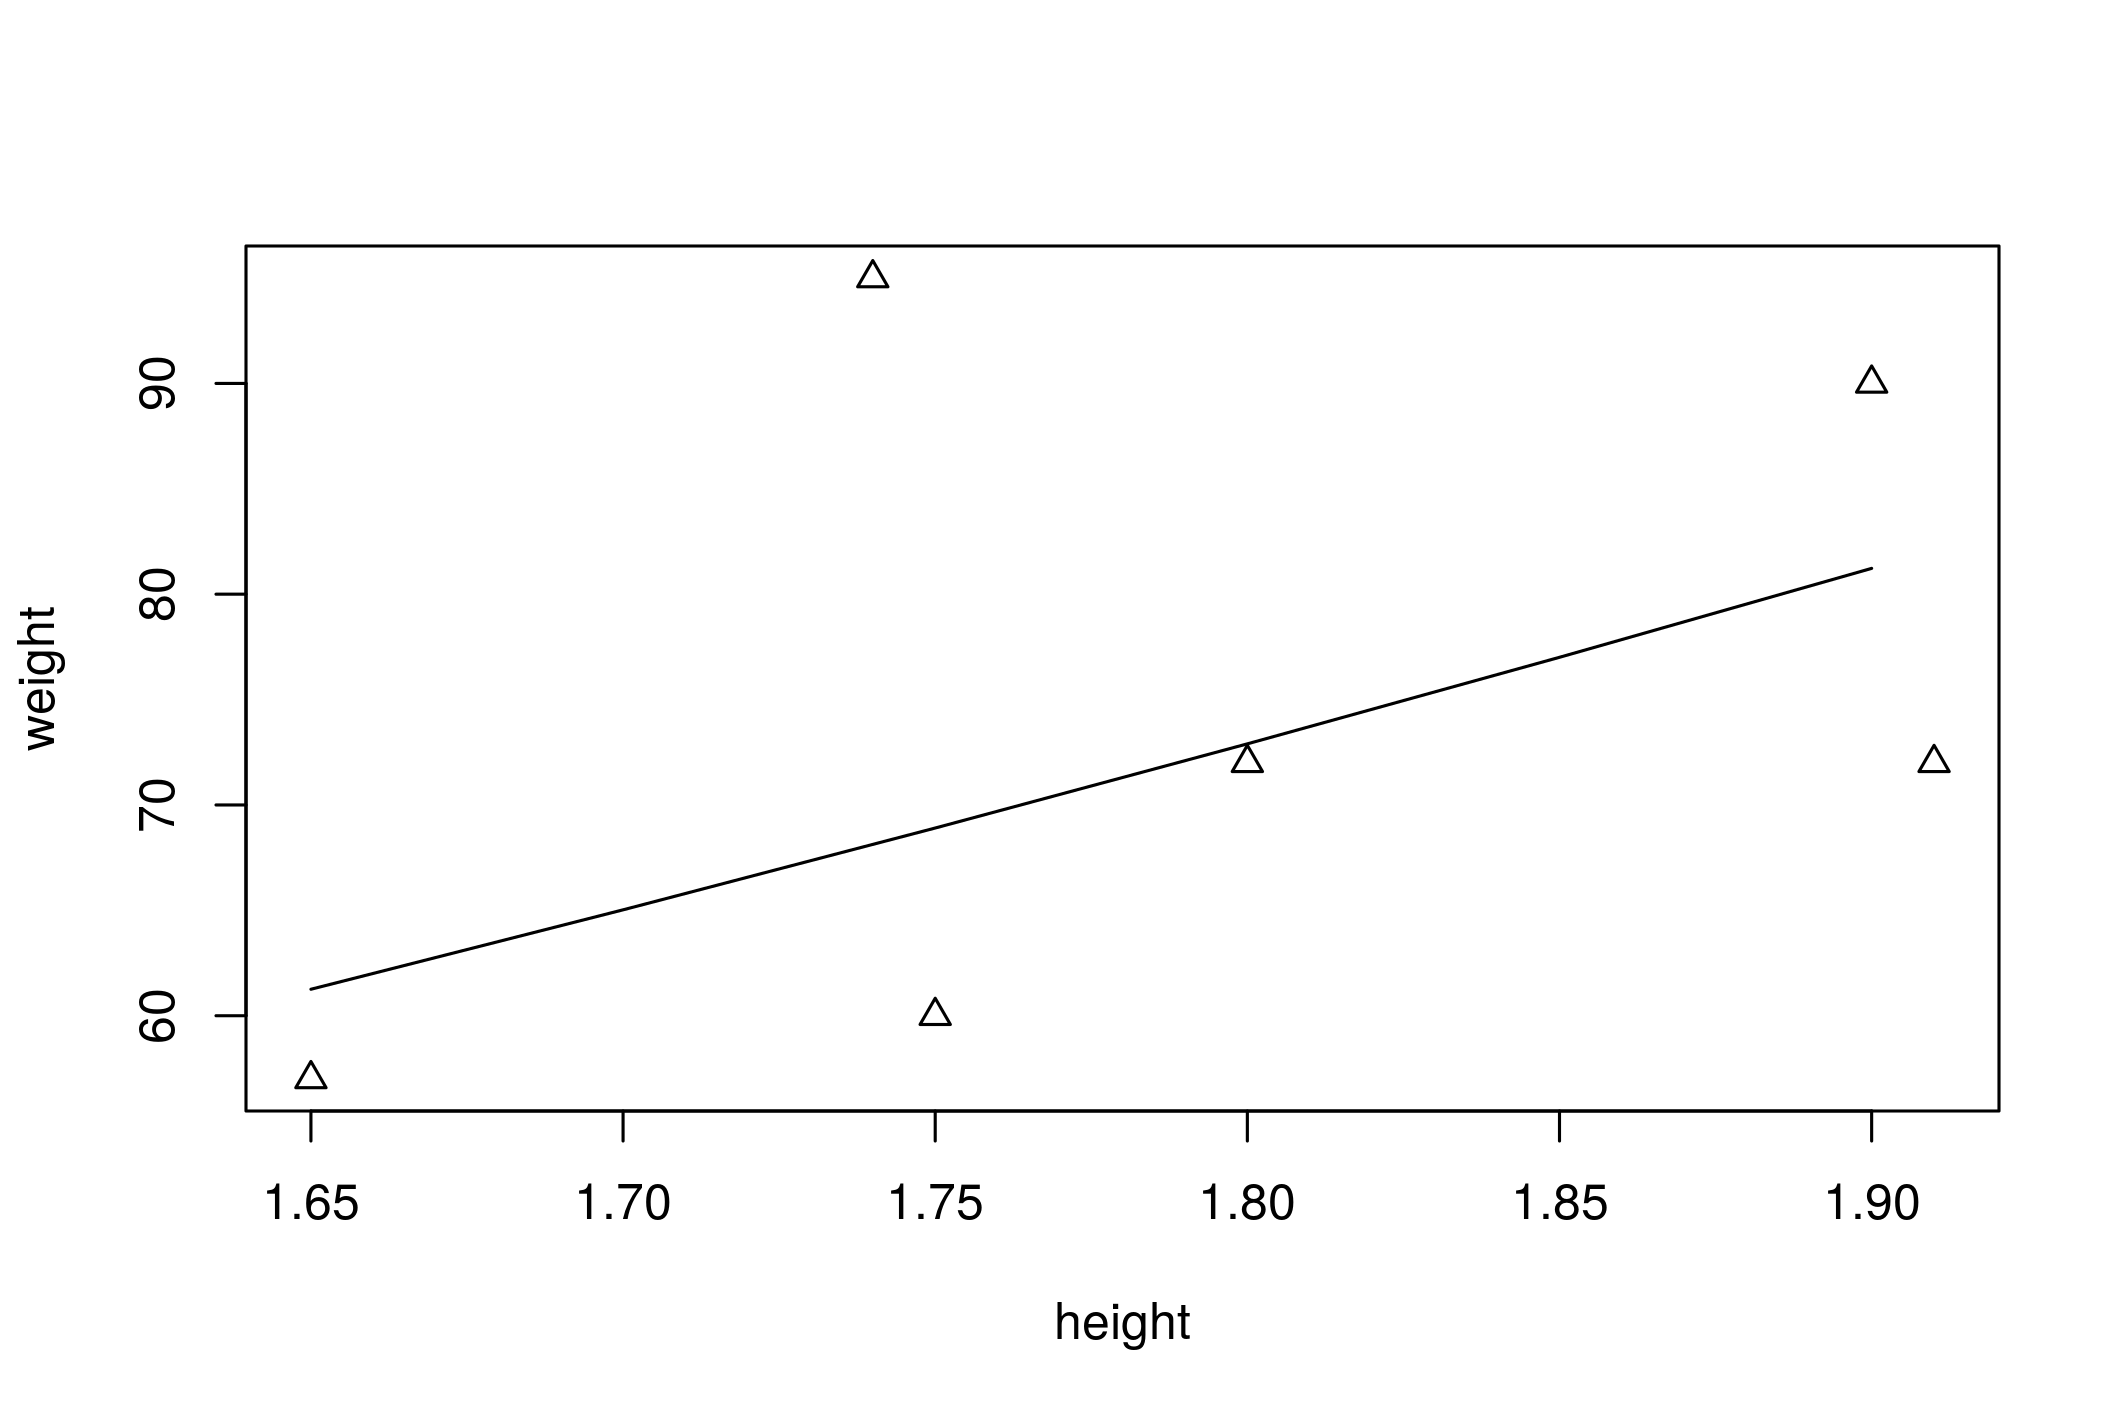
\includegraphics[width=0.95\textwidth]{fig-4.png}
	\caption{Sobreimponiendo una curva de referencia, usando \texttt{lines(...)}}
	\label{fig:fig-4}
\end{figure}
\newpage

Las expresiones suelen incluir referencias a variables, operadores como
\texttt{+} y llamadas de función, así como algunos otros elementos en los que
aún no hemos profundizado.  Las expresiones trabajan sobre objetos. Este es un
término abstracto para cualquier cosa que se pueda asignar a una variable. \textbf{R}
contiene varios tipos diferentes de objetos. Hasta ahora, hemos visto casi
exclusivamente vectores numéricos, pero en este capítulo introduciremos varios
tipos nuevos.  Aunque los objetos pueden ser explicados de forma abstracta,
sería una lectura bastante aburrida sin alguna indicación de cómo generarlos y
qué hacer con ellos. Por el contrario, gran parte de la sintaxis de las
expresiones tienen poco sentido sin conocer los objetos sobre los que se pretende
trabajar. Por lo tanto, las secciones siguientes alternan entre la introducción
de nuevos objetos y de nuevos elementos lingüísticos.

\subsection{Funciones y parámetros}

En este punto, ya tenemos una idea de la forma en que funciona \textbf{R}, y ya
hemos utilizado parte de una terminología especial cuando hablamos de la
función \texttt{plot}, etc. Ese es exactamente el punto: Muchas cosas en
\textbf{R} se hacen usando llamadas a funciones, comandos que parecen una
aplicación de una función matemática de una o varias variables; por ejemplo,
\texttt{log(x)} o \texttt{plot(height, weight)}. El formato es: un nombre de
función al cual le sigue un conjunto de paréntesis que contiene uno o más
parámetros. Por ejemplo, en \texttt{plot(height, weight)} el nombre de la
función es \texttt{plot} y los argumentos son \texttt{height} y
\texttt{weight}.  Estos son los parametros efectivos, que se usan en la
invocación final de la función, sin embargo una función también tiene
parámetros formales, que se conectan con parámetros reales en la invocación
final.

Cuando escribimos \texttt{plot(height , weight)}, \textbf{R} asume que el primer
parámetro corresponde a la variable \texttt{x} y el segundo a la variable
\texttt{y}. Esto se conoce como coincidencia posicional. Esto se vuelve difícil
de manejar si una función tiene un gran número de parámetros, ya que hay que
indicar cada uno de ellos y recordar su posición en la secuencia.
Afortunadamente, \textbf{R} tiene métodos para evitar esto: la mayoría de los
parámetros manejan valores por defecto y pueden omitirse en los casos de uso
comunes, y hay formas no posicionales de especificarlos cuando se necesita
apartarse de estos usos comunes.

La función \texttt{plot} es, de hecho, un ejemplo de una función que tiene una
gran variedad de parámetros para poder modificar símbolos, anchos de línea,
títulos, tipo de eje, etcétera. Usamos la forma alternativa de especificar
parámetros al establecer el símbolo de la gráfica en triángulos con
\texttt{plot(height, weight, pch=2)}. 

La forma \texttt{pch=2} se conoce como definición de parámetro por nombre, esta
forma permite la comparación de los parametros de llamada con los formales de
la función y por lo tanto permitie relacionar a ambos. La palabra clave
\texttt{pch} se utilizó para indicar que el parámetro corresponde con las
especificación del carácter de graficado. Esta forma de indicar cualquier
parámetro permite usar un orden arbitrario. De este modo, se puede escribir
\texttt{plot(x=height, y=weight)} y obtener el mismo gráfico que
\texttt{plot(y=weight, x=height)}.  

Los dos tipos de especificación de parametros --posicional y por nombre-- pueden
usarse al mismo tiempo. 

Aunque no haya parámetros para el llamado a una función, es necesario escribir
\texttt{ls()}, con los paréntesis, para mostrar el contenido del espacio de
trabajo. Un error común es olvidar escribir los paréntesis, lo que termina
provocando la visualización de un trozo de código \textbf{R} puesto que
\texttt{ls} (sin paréntesis) indica que se desea ver la definición de la
función en lugar de ejecutarla.

Los parámetros formales de una función forman parte de la definición de la
misma. El conjunto de los paramétros formales de una función, por ejemplo,
\texttt{plot.default} (que es la función que se llama cuando se le pasa a
\texttt{plot} un parámetro \texttt{x} porque no existe un método especial de
trazado), puede verse con:
\newpage

\begin{lstlisting}[language=R]
> args(plot.default)
function (x, y = NULL, type = "p", xlim = NULL, ylim = NULL,
log = "", main = NULL, sub = NULL, xlab = NULL, ylab = NULL,
ann = par("ann"), axes = TRUE, frame.plot = axes,
panel.first = NULL, panel.last = NULL, asp = NA, ...)
\end{lstlisting}

Note que la mayoría de los parámetros tienen valores por defecto, en el caso de
\texttt{type} si no lo especificamos, la función se comportará como si
hubieramos inidcado \texttt{type="p"}. El \texttt{NULL} por defecto para muchos
de los parámetros, realmente sirve como indicador que el mismo no se ha
especificado, permitiendo definir un comportamiento especial dentro de la
función. Por ejemplo, si no se especifican los parámetros \texttt{xlab} e
\texttt{ylab} estos se construyen a partir de los parametros reales pasados
como \texttt{x} e \texttt{y}. (Hay algunos puntos muy sutiles asociados con
esto, pero no vamos a profundizar más allá en el tema.)

El parámetro especial \texttt{(...)} -- Triple punto -- indica que esta función
aceptará parámetros adicionales cuyos nombres y cantidades no han sido
especificados aún de forma formal. Por lo general se usan para definir
parámetros que serán pasados a otras funciones, aunque algunas los traten de
forma particular.  Por ejemplo, en \texttt{data.frame} y \texttt{c}, los
parametros \texttt{...} representan el resultado recibido desde otra función.

\begin{lstlisting}[language=R]
# El resultado de matrix(1:4, nrow = 2) es la entrada de data.frame(...)
> df <- data.frame(matrix(1:4, nrow = 2)) 

  X1 X2
1  1  3
2  2  4
\end{lstlisting}

\subsection{Vectores}

Ya hemos visto vectores numéricos. Hay dos tipos más, vectores de caracteres y
vectores lógicos.

Un vector de caracteres es un vector de cadenas de texto cuyos elementos están
especificados entre comillas simples \texttt{'} o dobles \texttt{"}:

\begin{lstlisting}[language=R]
> c("Huey","Dewey","Louie")
[1] "Huey" "Dewey" "Louie"
\end{lstlisting}

No importa que comillas usemos, lo que es importante es que si la cadena
comienza con una finalice con la misma.

\begin{lstlisting}[language=R]
> c(\cite{Huey},\cite{Dewey}, \cite{Louie})
[1] "Huey" "Dewey" "Louie"
\end{lstlisting}

Sin embargo, debe evitar el uso del acento agudo \texttt{`}, que está presente
en algunos teclados. Usaremos las comillas dobles a lo largo de este libro para
evitar errores. Los vectores lógicos pueden tomar el valor \texttt{TRUE} o
\texttt{FALSE} (o \texttt{NA}; ver abajo). Tambien puede usar las abreviaturas
\texttt{T} y \texttt{F} (si tiene cuidado de no redefinirlas). Los vectores
lógicos se construyen usando la función \texttt{c} al igual que cualquier otros
tipo de vector:
\newpage

\begin{lstlisting}[language=R]
> c(T,T,F,T)
[1] TRUE TRUE FALSE TRUE
\end{lstlisting}

En realidad, es raro que tenga que especificar vectores lógicos de la manera
anterior. Es mucho más común usar valores lógicos únicos para activar o
desactivar una determinada opción en una llamada a una función. Los vectores de
más de un valor a menudo suelen ser el resultado de expresiones relacionales:


\begin{lstlisting}[language=R]
> bmi > 25
[1] FALSE FALSE FALSE FALSE TRUE FALSE
\end{lstlisting}

\subsection{Encomillado y secuencias de escape}

Las cadenas de caracteres entrecomilladas requieren algunas consideraciones
especiales: ¿Cómo, por ejemplo, que pasa si tenemos agregar una comilla dentro
de la cadena? ¿Y qué pasa con los caracteres especiales como el de fín de
linea? Este tipo de situaciones se resuelve usando secuencias de escape. Las
veremos inmediatamente, pero antes será útil observar lo siguiente.

Existe una diferencia entre una cadena de texto y la forma en que ésta se
imprime. Cuando, por ejemplo, se define una cadena como \texttt{"Huey"}, se
trata de una cadena de cuatro caracteres, no de seis. Las comillas no son
realmente parte de la cadena, sino que están ahí para que el sistema pueda
diferenciar entre una cadena y un nombre de variable.

Si imprime un vector de caracteres, normalmente se imprimirá con comillas
añadidas a cada elemento del mismo. Hay una manera de evitar esto, usando la
función de \texttt{cat}.  Por ejemplo,

\begin{lstlisting}[language=R]
> cat(c("Huey","Dewey","Louie"))
Huey Dewey Louie
\end{lstlisting}

Esto imprime las cadenas sin comillas, separadas por un espacio. No hay una
nueva línea que siga a la cadena, por lo que el símbolo (\texttt{>}) para la
siguiente entrada sigue directamente al final de la línea. (\textbf{Nota:}
cuando el vector de caracteres es impreso por \texttt{cat} no hay manera de
distinguir la diferencia entre este vector de tres elementos con un vector que
contuviera una simple cadena \texttt{"Huey Dewey Louie"}).

Para obtener el símbolo del sistema es necesario agregar específicamente el
caracter de salto de línea \texttt{\textbackslash{}n}

\begin{lstlisting}[language=R]
> cat(c("Huey","Dewey","Louie","\n"))
Huey Dewey Louie
>
\end{lstlisting}

Aquí hay un ejemplo de lo que se conoce como secuencia de escape. En realidad
representa un solo caracter, el linefeed (LF) o fín de línea, pero se
representa como dos caracteres. La barra invertida \textbackslash{} se conoce
como el \textit{carácter de escape}. En una forma similar, puede insertar una
comilla usando los caracteres \texttt{\"}, como en:

\begin{lstlisting}[language=R]
> cat("What is \"R\"?\n")
What is "R"?
> 
\end{lstlisting}

También hay maneras de insertar otros caracteres de control y glifos
especiales, pero nos llevaría demasiado tiempo discutirlo en detalle. Algo
importante, sin embargo: ¿Qué hay del caracter de escape en sí mismo?  Este
también debe ser escapado, así que para indicar una barra invertida, hay que
repetirla (\texttt{\textbackslash{}\textbackslash{}}). Es importante saber esto
en particular cuando cuando tengamos que especificar rutas de archivo en
Windows. Consulte también la Sección \ref{readtextfile}.

\subsection{Valores faltantes}

En el análisis real de datos, con frecuencia no disponemos de alguna
observación (el paciente no se presentó, un experimento falló, etc.). El
software estadístico necesita formas de hacer frente a esto. \textbf{R} permite
que los vectores contengan un valor especial llamado \texttt{NA}. Este valor se
traslada a los cálculos por lo que las operaciones con valores \texttt{NA}
darán como resultado otro \texttt{NA}. Hay algunos temas especiales asociados
con el manejo de estos valores; los trataremos a medida que lo necesitemos (ver
"valores faltantes" en el índice).

\subsection{Funciones que crean vectores}

En esta sección, presentaremos tres funciones \texttt{c}, \texttt{seq}, y
\texttt{rep}, todas se usan para crear vectores de diferentes formas.  La
primera \texttt{c}, ya la hemos visto. Es la abreviatura de ``concatenar'', que
es justamente lo que hace: juntar los elementos indicados del primero al último:

\begin{lstlisting}[language=R]
> c(42,57,12,39,1,3,4)
[1] 42 57 12 39 1 3 4
\end{lstlisting}

También podemos concatenar directamente vectores de distinta cantidad de elementos:

\begin{lstlisting}[language=R]
> x <- c(1, 2, 3)
> y <- c(10, 20)
> c(x, y, 5)
[1] 1 2 3 10 20 5
\end{lstlisting}

\begin{tradnote} Note que el vector \texttt{x} contiene 3 elementos, el vector
\texttt{y} dos, y \texttt{5} es un vector en sí mismo de un solo elemento
\end{tradnote} \newpage

De todas formas no necesitamos usar \texttt{c} para crear un vector de longitud
1. Muchos escriben \texttt{c(1)}, pero para \textbf{R} es exactamente lo mismo
que escribamos un simple \texttt{1}.

Es posible también, asignar un nombre a cada elemento de un vector. Esto
modifica luego la forma en que éste se mostrará:

\begin{lstlisting}[language=R]
> x <- c(red="Huey", blue="Dewey", green="Louie")
> x
    red    blue   green 
 "Huey" "Dewey" "Louie"
\end{lstlisting}

(En este caso si tiene sentido usar \texttt{c} incluso con vectores de un solo
elemento)

Los nombres pueden configurarse o leerse mediante la función \texttt{names}:

\begin{lstlisting}[language=R]
> names(x)
[1] "red"   "blue"  "green"
\end{lstlisting}

En el caso de los vectores, todos los elementos deben ser del mismo tipo. Si
concatenamos diferentes tipos de datos \textbf{R} convertira todos al tipo menos
restrictivo:

\begin{lstlisting}[language=R]
> c(FALSE, 3)
[1] 0 3
> c(pi, "abc")
[1] "3.14159265358979" "abc"
> c(FALSE, "abc")
[1] "FALSE" "abc"
\end{lstlisting}

Lo que ocurrió es, que los valores lógicos se convierten a valores \texttt{0/1}
o \texttt{"FALSE/TRUE"} y los números a una representación de tipo cadena.

La segunda función, \texttt{seq}("secuencia"), se usa para generar series de
números equidistantes. Al escribir esto:

\begin{lstlisting}[language=R]
> seq(4,9)
[1] 4 5 6 7 8 9
\end{lstlisting}

podemos ver claramente, que hemos creado un vector con los enteros del 4 al 9.
Si buscamos secuencias que "salten" de a 2 elementos, podríamos escribir:

\begin{lstlisting}[language=R]
> seq(4,10,2)
[1] 4 6 8 10
\end{lstlisting}

Frecuentemente son necesarios estos tipos de vectores, particlarmente para
gráficos. Por ejemplo, anteriormente usamos un vector
\texttt{c(1.65,1.70,1.75,1.80,1.85,1.90)} para definir un conjunto de alturas,
algo que eventualmente podríamos haber escrito como
\texttt{seq(1.65,1.90,0.05)} (La ventaja de usar \texttt{seq} es más que obvia
si eventualmente necesitaramos crear pasos de 1cm en vez de 5cm)

Una forma especial de definir una secuencia con pasos igual a 1 es la siguiente:

\begin{lstlisting}[language=R]
> 4:9
[1] 4 5 6 7 8 9
\end{lstlisting}

Lo anterior es exactamente igual a hacer \texttt{seq(4,9)}, simplemente es más
sencillo de leer.

La tercer función, \texttt{rep} ("replicar"), es usada para generar valores que
se repiten. Se puede usar de dos formas, dependiendo si el segundo parámetro es
un vector o un número

\begin{lstlisting}[language=R]
> oops <- c(7,9,13)
> rep(oops,3)
[1]  7  9 13  7  9 13  7  9 13
> rep(oops,1:3)
[1]  7  9  9 13 13 13
\end{lstlisting}

La primera de las ejecuciones repite completamente el vector \texttt{oops} tres veces.
La segunda llamada repite cada elemento la cantidad de veces definida en el
segundo vector \texttt{(1,2,3)}, es decir que el 7 se repetirá una vez, el 9 dos, y el
13 tres.

La función rep se usa habitualmente para hacer cosas como agurpar elementos: Si
sabemos que las primeras 10 observaciones son hombres y las últimas 17 mujeres,
podemos hacer:

\begin{lstlisting}[language=R]
> rep(1:2,c(10,15))
[1] 1 1 1 1 1 1 1 1 1 1 2 2 2 2 2 2 2 2 2 2 2 2 2 2 2
\end{lstlisting}

para armar un vector que nos indica que las observaciones corresponden a un
hombre (1) o a una mujer (2).  Una forma de repetir un mismo número de veces un
elemento, puede lograrse mediante \texttt{rep(1:2,each=10)} que es lo mismo que
hacer \texttt{rep(1:2,c(10,10))}.


\subsection{Matrices y arreglos}
\subsection{Factores}
\subsection{Listas}
\subsection{Data frames}
\subsection{Indexado}
\subsection{Selección condicional}
\subsection{Indexado de data frames}
\subsection{Agrupación de datos y data frames}
\subsection{Ciclos implícitos}
\subsection{Ordenamiento}


%%%%%%%%%%%%%%%%%%%%%%%%%%%%%%%%%%%%%%%%%%%%%%%%%%%%%%%%%%%%%%%%%%%%%%%%%%%%%%%
%% El Entorno de R
%%%%%%%%%%%%%%%%%%%%%%%%%%%%%%%%%%%%%%%%%%%%%%%%%%%%%%%%%%%%%%%%%%%%%%%%%%%%%%%
\chapter{El entorno de R}

\subsection{Leyendo desde un archivo de texto} \label{readtextfile}

\end{document}

